\documentclass[paper=a4, fontsize=11pt]{scrartcl} % A4 paper and 11pt font size
\usepackage[utf8]{inputenc}
\usepackage[T1]{fontenc} % Use 8-bit encoding that has 256 glyphs
\usepackage[english]{babel} % English language/hyphenation
\usepackage{amsmath,amsfonts,amsthm} % Math packages

\usepackage{graphicx}
\usepackage{siunitx}

\usepackage{amssymb}

\usepackage[nottoc]{tocbibind}

\usepackage[backend=bibtex]{biblatex}
\bibliography{bibtexlibs}

\usepackage{todonotes}

\usepackage{sectsty} % Allows customizing section commands
\allsectionsfont{\centering \normalfont\scshape} % Make all sections centered, the default font and small caps

\usepackage{fancyhdr} % Custom headers and footers
\pagestyle{fancyplain} % Makes all pages in the document conform to the custom headers and footers
\fancyhead[L]{} % No page header - if you want one, create it in the same way as the footers below
\fancyfoot[L]{} % Empty left footer
\fancyfoot[C]{} % Empty center footer
\fancyfoot[R]{\thepage} % Page numbering for right footer
\renewcommand{\headrulewidth}{0pt} % Remove header underlines
\renewcommand{\footrulewidth}{0pt} % Remove footer underlines
\setlength{\headheight}{13.6pt} % Customize the height of the header

\usepackage{hyperref}
\hypersetup{
    colorlinks,
    citecolor=black,
    filecolor=black,
    linkcolor=black,
    urlcolor=black
}

\fancypagestyle{firststyle}
{
  \fancyhf{}
  \fancyfoot[R]{\thepage}
}

\numberwithin{equation}{chapter} % Number equations within chapters (i.e. 1.1, 1.2, 2.1, 2.2 instead of 1, 2, 3, 4)
\numberwithin{figure}{chapter} % Number figures within chapters (i.e. 1.1, 1.2, 2.1, 2.2 instead of 1, 2, 3, 4)
\numberwithin{table}{chapter} % Number tables within chapters (i.e. 1.1, 1.2, 2.1, 2.2 instead of 1, 2, 3, 4)

%------ Listings --------------
\usepackage{color}
\definecolor{light-gray}{gray}{0.95}
\definecolor{orange}{rgb}{1, 0.5, 0}
\usepackage{listings}
\usepackage{mips}

\lstnewenvironment{code}[1][]%
{\minipage{\linewidth}
\lstset{ %
language={[mips]Assembler},  % choose the language of the code
basicstyle=\footnotesize,       % the size of the fonts that are used for the code
numbers=left,                   % where to put the line-numbers
numberstyle=\footnotesize,      % the size of the fonts that are used for the line-numbers
stepnumber=1,                   % the step between two line-numbers. If it is 1 each line will be numbered
resetmargins=true,              % reset line numbers
numbersep=5pt,                  % how far the line-numbers are from the code
backgroundcolor=\color{white},  % choose the background color. You must add \usepackage{color}
showspaces=false,               % show spaces adding particular underscores
showstringspaces=false,         % underline spaces within strings
showtabs=false,                 % show tabs within strings adding particular underscores
frame=single,                   % adds a frame around the code
tabsize=2,                      % sets default tabsize to 2 spaces
captionpos=b,                   % sets the caption-position to bottom
breaklines=true,                % sets automatic line breaking
breakatwhitespace=false,        % sets if automatic breaks should only happen at whitespace
escapeinside={\%*}{*)},         % if you want to add a comment within your code
identifierstyle=\color{blue},
stringstyle=\color{orange},
firstnumber=0,
#1
}}%
{\endminipage}


%----------------------------------------------------------------------------------------
%   TITLE SECTION
%----------------------------------------------------------------------------------------

\newcommand{\horrule}[1]{\rule{\linewidth}{#1}} % Create horizontal rule command with 1 argument of height

\title{ 
\normalfont \normalsize 
\textsc{Norwegian University of Science and Technology} \\ [25pt] % Your university, school and/or department name(s)
\horrule{0.5pt} \\[0.4cm] % Thin top horizontal rule
\huge \textbf{Assignment 1} \\ % The assignment title
TDT4255 \\
\horrule{2pt} \\[0.5cm] % Thick bottom horizontal rule
}

\author{Authors:\\Aleksander V. Burkow\\Stian Jensen\\Christoffer Tønnessen}

\date{\normalsize\today}

\begin{document}

\pagenumbering{roman}

\maketitle

\thispagestyle{firststyle}

\newpage

%ABSTRACT
\section*{Abstract}
\label{sec:abstract}

\vspace*{\fill}
This report presents a solution to the first assignment for the subject TDT4255 at NTNU.
A small multi cycle processor was written in VHDL for the Xilinx Spartan-6 FPGA.
A subset of the MIPS instruction set was successfully implemented and ran on the FPGA.
The generated processors clock frequence far exceeds the defined 24 MHz on the FPGA.
\vspace*{\fill}


\newpage

\tableofcontents

\setcounter{secnumdepth}{3}

\newpage

\pagenumbering{arabic}

%INTRODUCTION
\section{Introduction}

Introduction and a citation \cite{example} .


\newpage

%SOLUTION
\chapter{Solution}

% Solution: describes your solution of the task.
% Contains a detailed description of all the subtasks which have been solved and how they contribute to the solution for the given task.
% The use of diagrams, figures, tables and similar is welcome as a support to your description.

\section{Architecture}

Data hazards, control hazards, structural hazards.

The design of the processor is based on the architecture provided in Figure 5.1 \cite[p. 50]{compendium}.
It has been extended to support jumps, data forwarding, hazard detection and branch prediction.

\section{Implementation}

\subsection{Data Forwarding}

\subsection {Hazard Detection}
The implemented data forwarding will not be able to handle all kinds of data hazards.
Specifically, an R-type instruction directly following a load instruction, where the load's destination register is one of the source registers of the R-type instruction, can not benefit from data forwarding.
This is because while the R-type instruction is in the execute stage, the load instruction is still only in the MEM stage, and the data will not be ready before the next cycle.

To work around this issue, a hazard detection unit will detect a load followed by a data-dependent instruction (this does not apply to store instructions, as data forwarding takes care of this case).
A stall flag is enabled when a load instruction is currently in its execute stage, while a dependent instruction is in the ID stage.
This causes the dependent instruction to remain in the ID stage for one extra cycle, while the load instruction progresses to the MEM stage.
To give the effect of a nop (an instruction which does not alter memory) between them, the control signals for the dependent instruction are set to zero for one cycle.
At the same time, the PC needs to stall for one cycle, so no instructions are skipped.
The next clock cycle, the instruction enters the execute stage.
Then, data will be loaded from memory, residing in the WB stage, where we have already implemented data forwarding to the EX stage.

\subsection{Branching}

This processor implements multiple branch-related improvements compared to a naïve pipelined datapath. These improvements allow for speculative execution of instructions, keeping the pipeline full at all times.

The improvements include:
\begin{enumerate}
  \item
    Moving branch decisions from the memory stage to the instruction decode stage, comparing register values in a dedicated equality unit.
    This allows for instant branches with no lost cycles when data hazards are absent.
  \item
    When operands are unavailable in the ID stage, one cannot decide whether to take the branch.
    By making an educated guess using a branch prediction unit (containing a two-bit predictor\todo{cite a two bit predictor explained somewhere else so we dont have to? Or should we explain it}) we can speculatively execute instructions, keeping the pipeline filled.
    If a branch is taken wrongly, only two pipeline stages have to be flushed, always netting an improvement over delayed branching.
\end{enumerate}

To allow for zero-downtime branching, the program counter allows for instant updates, implemented via an internal bypass straight through to the instruction memory.
This allows us to update the PC to the target branch address the same cycle we decide to branch, thereby having the branch-target instruction ready at the next clock cycle.

To correct for wrongly taken branches, all branch related signals (branch\_taken, control\_should\_branch, and branch\_pc\_not\_taken) are passed on through the pipeline.
In the MEM stage, when the branch operands actually have been compared, corrective action can be taken if the wrong choice was made.
If there was a choice to branch, and the branch taken signal and alu result zero flag differ, the branch was taken wrongly.
Pipeline stages ID and EX have to be flushed, as well as the pc reset to the address of the pc not taken (branch\_pc\_not\_taken).
Afterwards, execution resumes as normal, having lost only two cycles if the branch was predicted wrongly.

There are multiple ways to decide on which choice to predict.
\todo{This entire bit. finish it}
STATIC BRANCHING VERSUS DYNAMIC
This data is also fed back to the branch prediction unit, allowing the two bit predictor to learn from recent branch behaviour to give better predictions in the future.
tradeoff critical path thru branch predictor


\clearpage

%TESTS&RESULTS
\chapter{Tests \& Results}

\section{Tests}

This section presents highlights from the testing suite of the pipelined MIPS processor with speculative execution. Branch prediction, data forwarding (including load-store forwarding), and pipeline flushing is demonstrated executing successfully.

\subsection{System integration test}

The provided system integration test from exercise 1,\todo{Add reference?}
which tests basic load, store, jump and arithmetic, was successfully run on the pipelined architecture.
The testbench has been extended to be more thorough, checking that the data from store
instructions following a branch taken doesn't end up in memory.

\subsection{Store after load operand forwarding}

The presented architecture has been extended to support operand forwarding from the write-back pipeline stage to the memory stage.
This allows for load instructions to be followed by store instructions without having to insert pipeline bubbles.

\begin{figure}[h]
  \begin{code}
    lui $3, 2
    srl $3, $3, 16   # Load 2 to $3
    lw $3, 1($0)     # Loads 1 from memory
    sw $3, 3($0)     # Should store 1, not 2 to address 3
  \end{code}
  \caption{Assembly to test store after load operand forwarding}
  \label{fig:test-store-after-load}
\end{figure}

Expected behavior:
\begin{itemize}
  \item
    The sw instruction should store the newly loaded value from the lw instruction, in effect acting like a memory move instruction.
  \item
    Bubbles should not be inserted into the pipeline.
\end{itemize}

\subsection{Branch prediction}

The test case in figure \ref{fig:test-branch-prediction} tests both the hazard detection and branch prediction capabilities of the processor.

\begin{figure}[h]
  \begin{code}
    lw $1, 0($0)
    lw $2, 1($0)      # Should stall after this instruction (data hazard).
    beq $2, $0, 3     # Should predict (Control hazard).
    sw $2, 2($0)
    sub $2, $2, $1    # Introduce data hazard for beq
    j 2               # Jump to loop condition
    beq $0, $0, -1    # Loop forever
  \end{code}
  \caption{Assembly to test branch prediction} \label{fig:test-branch-prediction}
\end{figure}

Expected behavior:
\begin{itemize}
  \item
    The pipeline stalling on instruction 2. Branch after load requires one stall cycle to actually be able to correct for wrongly taken branches.
  \item
    The processor predicting whether instruction 2 should branch or not.
    Operands are available neither the first time (load not having completed yet), or after the end-of-loop jump (the sub instruction not having completed yet).
    As this architecture doesn't support operand forwarding to the branch predictor, it will have to guess.
\end{itemize}


\subsection{Pipeline flushing}

The test case in figure \ref{fig:test-pipeline-flushing} tests that speculatively executed instructions are correctly flushed from the pipeline.

\begin{figure}[h]
  \begin{code}
    lw $2, 2($0)    # Loads 2 into $2
    lw $1, 1($0)    # Loads 1 into $1
    beq $1, $0, 2   # Branch speculatively not taken
    sw $2, 4($0)    # Speculatively executed, to be flushed
    j 6             # Speculatively executed, to be flushed
    sw $1, 4($0)    # Should actually be executed
  \end{code}
  \caption{Assembly to test pipeline flushing}
  \label{fig:test-pipeline-flushing}
\end{figure}

Expected behavior:
\begin{itemize}
  \item
    Instructions 3 and 4 should be speculatively executed, and flushed.
  \item
    The value from memory address 1, not 2 should end up at memory address 4.
\end{itemize}

\section{Component Tests}

\begin{table}[h!]
    \begin{tabular}{|l|p{9cm}|l|}
    \hline
    \textbf{Unit under test} & \textbf{Test purpose}               & \textbf{Test status} \\ \hline
    PC                & Does the program counter increment normally? & \checkmark Passed \\ \cline{2-2}
                      & Can the program counter be paused? & \\ \cline{2-2}
                      & Is the correct order of overrides respected (branch predict, jump, branch correct)? & \\ \hline
    Forwarding unit   & Can data be forwarded from MEM stage to EX stage? & \checkmark Passed \\ \cline{2-2}
                      & Can data be forwarded from WB stage to EX stage? & \\ \cline{2-2}
                      & Can data be forwarded from WB stage to MEM stage? & \\ \cline{2-2}
                      & Is \$r0? ignored & \\ \cline{2-2}
                      & Will it incorrectly forward when control\_reg\_write is not enabled? & \\ \hline
    Two bit predictor & Confirm that the predictor defaults to 'not taken'. & \checkmark Passed \\ \cline{2-2}
                      & Check that two missed predictions are required before prediction switches. & \\\cline{2-2}
                      & Confirm that it properly resets to 'not taken'. & \\ \hline
    Hazard detection  & Confirm that the pipeline doesn't stall when an r-type instruction follows a load, but there's no overlap in registers & \checkmark Passed \\ \cline{2-2}
                      & Check that the pipeline stalls when a memory read precedes a dependent r-type or branch instruction. & \\\cline{2-2}
                      & Check that the pipeline doesn't stall when a data-dependent store instruction follows a load instruction. & \\ \hline
    Control unit      & Confirm that appropriate control signals are output for all supported instructions. & \checkmark Passed \\ \cline{2-2}
                      & Confirm that all outputs are zero when processor is not enabled. & \\ \hline
    \end{tabular}
    \caption{VHDL component tests}
    \label{fig:vhdl_component_tests}
\end{table}


\clearpage

%DISCUSSION
\chapter{Discussion}

\section{Requirements}
The major requirement, to implement a simple 5-stage pipelined processor was met.
Furthermore, the solution includes a data forwarding unit, a hazard detector, and a dynamic 2-bit branch predictor.
It has been successfully tested on a Xilinx Spartan-6 LX16 FPGA, using the provided hostcomm\cite{hostcomm} utility.

\section{Performance}

The final estimated clock frequency is 62.38 MHz.
This is mostly due to a long critical path introduced by having a branch predictor and a forwarding unit.
However, the pipelined processor gives a tremendous increase in instruction throughput.

The critical path is introduced by having a forwarding unit.
To reduce the path, one could remove the unit.
If this is done there will be a lot of data hazards, which will mean that the processor has to stall a lot of the time.
It is not reasonable to believe that the higher clock frequence achieved from removing the forwarding unit, but with a lot of new stalls, will make programs run faster.
This might be the case in a program with no data hazards, but this is not the case in most programs.

When comparing to the multi-cycle processor we implemented in assignment 1, we see that the number of cycles required to execute the provided test program is reduced from 98 to 29.
And although the clock frequency has been somewhat reduced after introducing pipelining, it still represents a speedup of about 2.78.


\section{Choosing a branch predictor}
The choice of using a single shared saturating counter versus a predictor table indexed by the low bits of the current instruction, was based on noticing that programs usually were rather short, containing at most a few tight loops.

As this architecture doesn't support data forwarding to the branch predictor, even the addition of a single two bit predictor reduces pipeline flushing in loops dramatically, as the previous loop condition can be re-used and will be correct for all loop iterations except the last.

\section{The Work Process}
We decided to take a gradual approach to the assignment.
The first stage was to convert the processor from Assignment 1 into a processor with five pipeline stages, and modified the test program to have enough nops to remove all hazards.

With this implementation working, we could progress to add data forwarding, and observe that the test passed with significantly fewer nops required.
This approach let us test each new component's integration in the system before progressing to the new task, until finally the original test program ran to completion.

\section{Further Work}

The branch prediction unit can be extended quite easily.
As the current implementation uses a single shared two bit predictor, it is ill suited for larger programs with more complex branching behaviour.
If one wishes to support such programs, one can use a table of two bit predictors indexed by the current pc to get more finegrained prediction.

With the addition of a global predictor, that is a table of two-bit predictors indexed by the last five branching decisions, complex behavior resulting from correlating branches can also be captured.
Combining these global and local predictors, choosing between them with a toplevel two bit predictor, tournament prediction has been reinvented.


\clearpage

%CONCLUSION
\section{Conclusion}

% Conclusion: a brief conclusion of the performed work.
% Round up the challenges and results.

All requirements given in the assignment were completed.
In addition, the processor is fairly efficient as several optimizations has been made after completing the initial design.

Our approach of first implementing support for the required instructions, and confirming that they fork on the FPGA, before making optimizations and adding extra instructions proved to be smart.
In the end, there was time for profiling of the processor to identify bottlenecks.
Removing the largest bottlenecks ended up increasing the clock frequency to 73.573MH.

The most difficult part of this assignment was getting familiar with writing VHDL code.
Writing small components by themselves and testing them with testbenches was easy enough,
but inspecting the generated RTL often showed that the written VHDL did not properly describe the intended components.
In addition, testing the final processor design was quite tedious, as there were many signals to keep track of to figure out where the processor diverged from desired behavior.

In conclusion, it was a challenging and educational assignment.
Things learned from it will be helpful both in the next assignment as well as in the course TDT4295.


\clearpage

\printbibliography

\newpage

\begin{alphasection}
%APPENDIX A
\section{Appendix A}

\begin{figure}[ht!]
    \begin{center}
    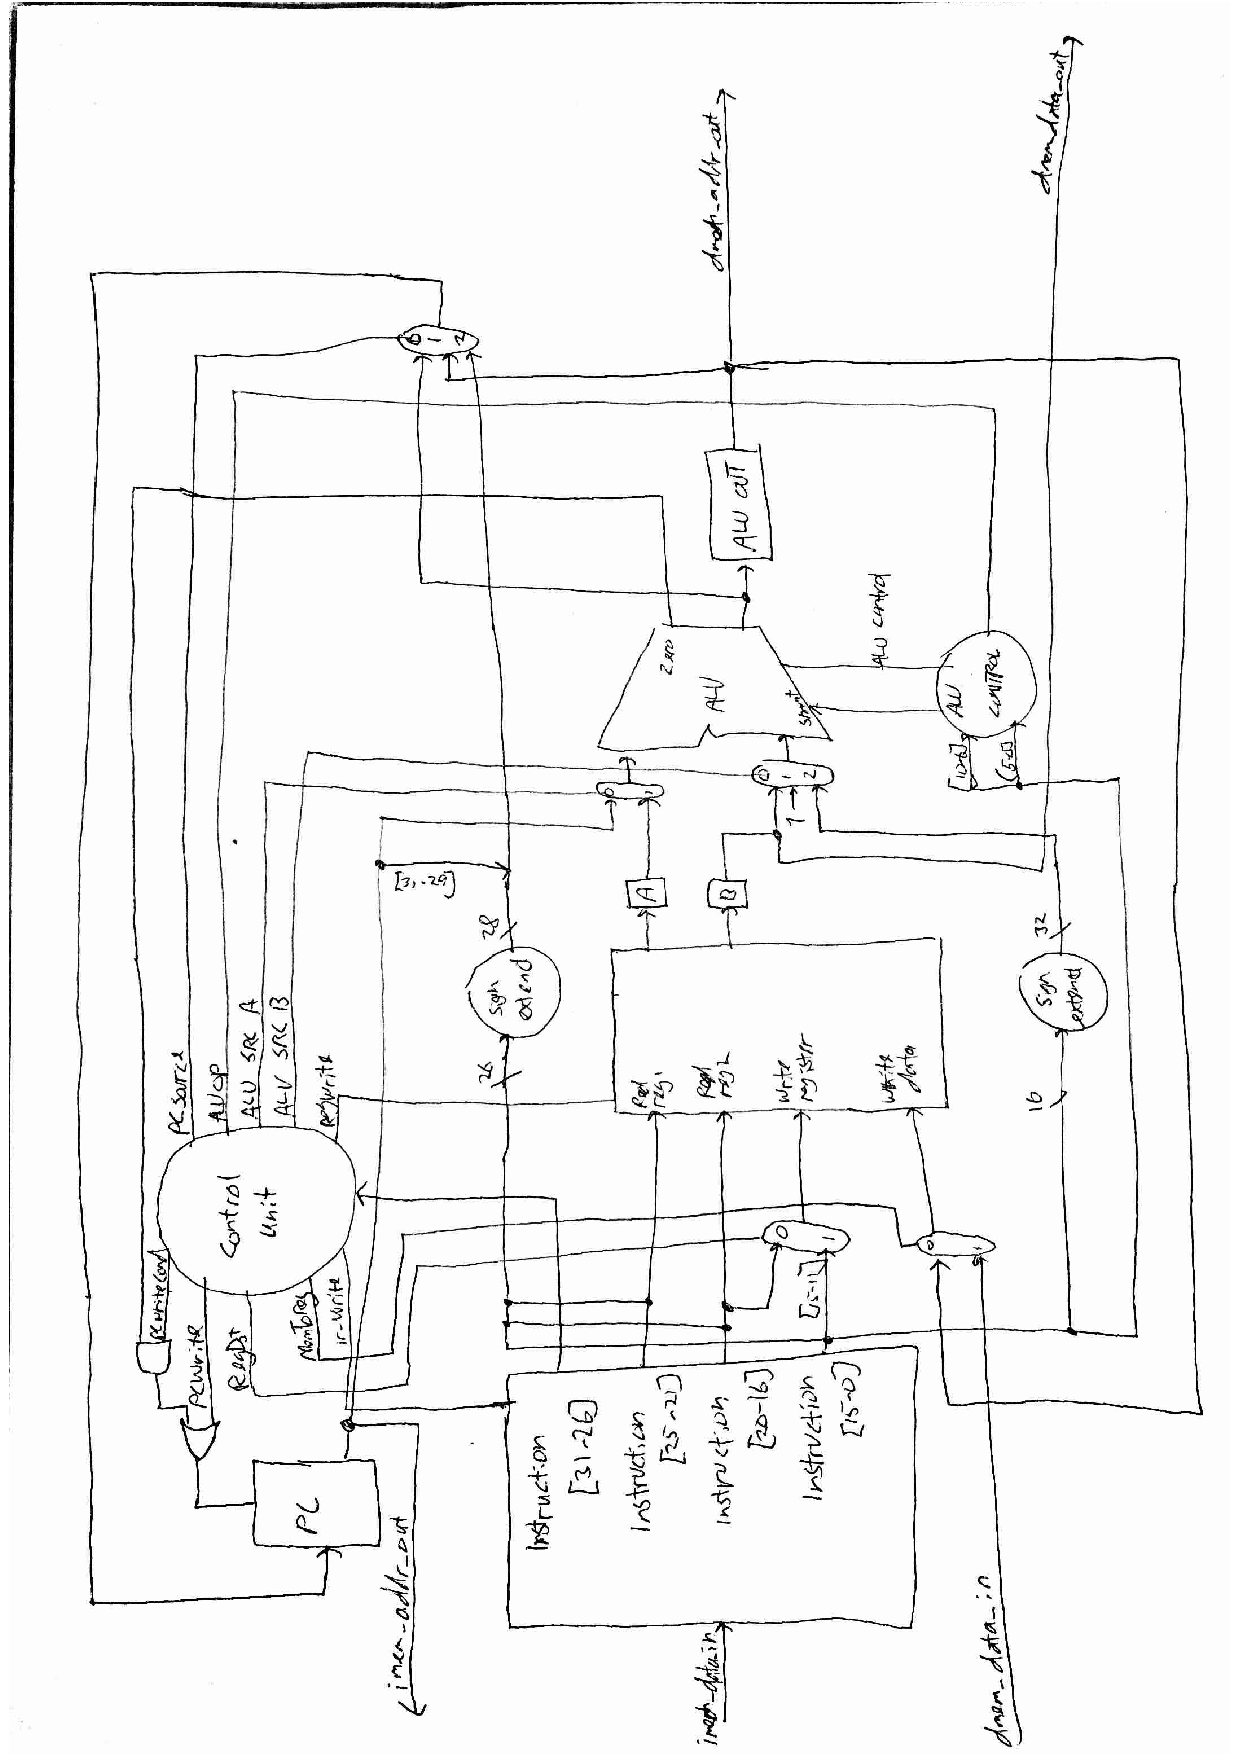
\includegraphics[width=\textwidth]{assets/top_level_rtl.pdf}
    \caption{Top level RTL schematic}
    \label{fig:top_level_rtl}
    \end{center}
\end{figure}


\end{alphasection}

\end{document}
